
\documentclass[10pt]{article} % For LaTeX2e
\usepackage{iclr2025_conference}
\usepackage{times}

\iclrfinalcopy

% Optional math commands from https://github.com/goodfeli/dlbook_notation.
%%%%% NEW MATH DEFINITIONS %%%%%

\usepackage{amsmath,amsfonts,bm}

% Mark sections of captions for referring to divisions of figures
\newcommand{\figleft}{{\em (Left)}}
\newcommand{\figcenter}{{\em (Center)}}
\newcommand{\figright}{{\em (Right)}}
\newcommand{\figtop}{{\em (Top)}}
\newcommand{\figbottom}{{\em (Bottom)}}
\newcommand{\captiona}{{\em (a)}}
\newcommand{\captionb}{{\em (b)}}
\newcommand{\captionc}{{\em (c)}}
\newcommand{\captiond}{{\em (d)}}

% Highlight a newly defined term
\newcommand{\newterm}[1]{{\bf #1}}


% Figure reference, lower-case.
\def\figref#1{figure~\ref{#1}}
% Figure reference, capital. For start of sentence
\def\Figref#1{Figure~\ref{#1}}
\def\twofigref#1#2{figures \ref{#1} and \ref{#2}}
\def\quadfigref#1#2#3#4{figures \ref{#1}, \ref{#2}, \ref{#3} and \ref{#4}}
% Section reference, lower-case.
\def\secref#1{section~\ref{#1}}
% Section reference, capital.
\def\Secref#1{Section~\ref{#1}}
% Reference to two sections.
\def\twosecrefs#1#2{sections \ref{#1} and \ref{#2}}
% Reference to three sections.
\def\secrefs#1#2#3{sections \ref{#1}, \ref{#2} and \ref{#3}}
% Reference to an equation, lower-case.
\def\eqref#1{equation~\ref{#1}}
% Reference to an equation, upper case
\def\Eqref#1{Equation~\ref{#1}}
% A raw reference to an equation---avoid using if possible
\def\plaineqref#1{\ref{#1}}
% Reference to a chapter, lower-case.
\def\chapref#1{chapter~\ref{#1}}
% Reference to an equation, upper case.
\def\Chapref#1{Chapter~\ref{#1}}
% Reference to a range of chapters
\def\rangechapref#1#2{chapters\ref{#1}--\ref{#2}}
% Reference to an algorithm, lower-case.
\def\algref#1{algorithm~\ref{#1}}
% Reference to an algorithm, upper case.
\def\Algref#1{Algorithm~\ref{#1}}
\def\twoalgref#1#2{algorithms \ref{#1} and \ref{#2}}
\def\Twoalgref#1#2{Algorithms \ref{#1} and \ref{#2}}
% Reference to a part, lower case
\def\partref#1{part~\ref{#1}}
% Reference to a part, upper case
\def\Partref#1{Part~\ref{#1}}
\def\twopartref#1#2{parts \ref{#1} and \ref{#2}}

\def\ceil#1{\lceil #1 \rceil}
\def\floor#1{\lfloor #1 \rfloor}
\def\1{\bm{1}}
\newcommand{\train}{\mathcal{D}}
\newcommand{\valid}{\mathcal{D_{\mathrm{valid}}}}
\newcommand{\test}{\mathcal{D_{\mathrm{test}}}}

\def\eps{{\epsilon}}


% Random variables
\def\reta{{\textnormal{$\eta$}}}
\def\ra{{\textnormal{a}}}
\def\rb{{\textnormal{b}}}
\def\rc{{\textnormal{c}}}
\def\rd{{\textnormal{d}}}
\def\re{{\textnormal{e}}}
\def\rf{{\textnormal{f}}}
\def\rg{{\textnormal{g}}}
\def\rh{{\textnormal{h}}}
\def\ri{{\textnormal{i}}}
\def\rj{{\textnormal{j}}}
\def\rk{{\textnormal{k}}}
\def\rl{{\textnormal{l}}}
% rm is already a command, just don't name any random variables m
\def\rn{{\textnormal{n}}}
\def\ro{{\textnormal{o}}}
\def\rp{{\textnormal{p}}}
\def\rq{{\textnormal{q}}}
\def\rr{{\textnormal{r}}}
\def\rs{{\textnormal{s}}}
\def\rt{{\textnormal{t}}}
\def\ru{{\textnormal{u}}}
\def\rv{{\textnormal{v}}}
\def\rw{{\textnormal{w}}}
\def\rx{{\textnormal{x}}}
\def\ry{{\textnormal{y}}}
\def\rz{{\textnormal{z}}}

% Random vectors
\def\rvepsilon{{\mathbf{\epsilon}}}
\def\rvtheta{{\mathbf{\theta}}}
\def\rva{{\mathbf{a}}}
\def\rvb{{\mathbf{b}}}
\def\rvc{{\mathbf{c}}}
\def\rvd{{\mathbf{d}}}
\def\rve{{\mathbf{e}}}
\def\rvf{{\mathbf{f}}}
\def\rvg{{\mathbf{g}}}
\def\rvh{{\mathbf{h}}}
\def\rvu{{\mathbf{i}}}
\def\rvj{{\mathbf{j}}}
\def\rvk{{\mathbf{k}}}
\def\rvl{{\mathbf{l}}}
\def\rvm{{\mathbf{m}}}
\def\rvn{{\mathbf{n}}}
\def\rvo{{\mathbf{o}}}
\def\rvp{{\mathbf{p}}}
\def\rvq{{\mathbf{q}}}
\def\rvr{{\mathbf{r}}}
\def\rvs{{\mathbf{s}}}
\def\rvt{{\mathbf{t}}}
\def\rvu{{\mathbf{u}}}
\def\rvv{{\mathbf{v}}}
\def\rvw{{\mathbf{w}}}
\def\rvx{{\mathbf{x}}}
\def\rvy{{\mathbf{y}}}
\def\rvz{{\mathbf{z}}}

% Elements of random vectors
\def\erva{{\textnormal{a}}}
\def\ervb{{\textnormal{b}}}
\def\ervc{{\textnormal{c}}}
\def\ervd{{\textnormal{d}}}
\def\erve{{\textnormal{e}}}
\def\ervf{{\textnormal{f}}}
\def\ervg{{\textnormal{g}}}
\def\ervh{{\textnormal{h}}}
\def\ervi{{\textnormal{i}}}
\def\ervj{{\textnormal{j}}}
\def\ervk{{\textnormal{k}}}
\def\ervl{{\textnormal{l}}}
\def\ervm{{\textnormal{m}}}
\def\ervn{{\textnormal{n}}}
\def\ervo{{\textnormal{o}}}
\def\ervp{{\textnormal{p}}}
\def\ervq{{\textnormal{q}}}
\def\ervr{{\textnormal{r}}}
\def\ervs{{\textnormal{s}}}
\def\ervt{{\textnormal{t}}}
\def\ervu{{\textnormal{u}}}
\def\ervv{{\textnormal{v}}}
\def\ervw{{\textnormal{w}}}
\def\ervx{{\textnormal{x}}}
\def\ervy{{\textnormal{y}}}
\def\ervz{{\textnormal{z}}}

% Random matrices
\def\rmA{{\mathbf{A}}}
\def\rmB{{\mathbf{B}}}
\def\rmC{{\mathbf{C}}}
\def\rmD{{\mathbf{D}}}
\def\rmE{{\mathbf{E}}}
\def\rmF{{\mathbf{F}}}
\def\rmG{{\mathbf{G}}}
\def\rmH{{\mathbf{H}}}
\def\rmI{{\mathbf{I}}}
\def\rmJ{{\mathbf{J}}}
\def\rmK{{\mathbf{K}}}
\def\rmL{{\mathbf{L}}}
\def\rmM{{\mathbf{M}}}
\def\rmN{{\mathbf{N}}}
\def\rmO{{\mathbf{O}}}
\def\rmP{{\mathbf{P}}}
\def\rmQ{{\mathbf{Q}}}
\def\rmR{{\mathbf{R}}}
\def\rmS{{\mathbf{S}}}
\def\rmT{{\mathbf{T}}}
\def\rmU{{\mathbf{U}}}
\def\rmV{{\mathbf{V}}}
\def\rmW{{\mathbf{W}}}
\def\rmX{{\mathbf{X}}}
\def\rmY{{\mathbf{Y}}}
\def\rmZ{{\mathbf{Z}}}

% Elements of random matrices
\def\ermA{{\textnormal{A}}}
\def\ermB{{\textnormal{B}}}
\def\ermC{{\textnormal{C}}}
\def\ermD{{\textnormal{D}}}
\def\ermE{{\textnormal{E}}}
\def\ermF{{\textnormal{F}}}
\def\ermG{{\textnormal{G}}}
\def\ermH{{\textnormal{H}}}
\def\ermI{{\textnormal{I}}}
\def\ermJ{{\textnormal{J}}}
\def\ermK{{\textnormal{K}}}
\def\ermL{{\textnormal{L}}}
\def\ermM{{\textnormal{M}}}
\def\ermN{{\textnormal{N}}}
\def\ermO{{\textnormal{O}}}
\def\ermP{{\textnormal{P}}}
\def\ermQ{{\textnormal{Q}}}
\def\ermR{{\textnormal{R}}}
\def\ermS{{\textnormal{S}}}
\def\ermT{{\textnormal{T}}}
\def\ermU{{\textnormal{U}}}
\def\ermV{{\textnormal{V}}}
\def\ermW{{\textnormal{W}}}
\def\ermX{{\textnormal{X}}}
\def\ermY{{\textnormal{Y}}}
\def\ermZ{{\textnormal{Z}}}

% Vectors
\def\vzero{{\bm{0}}}
\def\vone{{\bm{1}}}
\def\vmu{{\bm{\mu}}}
\def\vtheta{{\bm{\theta}}}
\def\va{{\bm{a}}}
\def\vb{{\bm{b}}}
\def\vc{{\bm{c}}}
\def\vd{{\bm{d}}}
\def\ve{{\bm{e}}}
\def\vf{{\bm{f}}}
\def\vg{{\bm{g}}}
\def\vh{{\bm{h}}}
\def\vi{{\bm{i}}}
\def\vj{{\bm{j}}}
\def\vk{{\bm{k}}}
\def\vl{{\bm{l}}}
\def\vm{{\bm{m}}}
\def\vn{{\bm{n}}}
\def\vo{{\bm{o}}}
\def\vp{{\bm{p}}}
\def\vq{{\bm{q}}}
\def\vr{{\bm{r}}}
\def\vs{{\bm{s}}}
\def\vt{{\bm{t}}}
\def\vu{{\bm{u}}}
\def\vv{{\bm{v}}}
\def\vw{{\bm{w}}}
\def\vx{{\bm{x}}}
\def\vy{{\bm{y}}}
\def\vz{{\bm{z}}}

% Elements of vectors
\def\evalpha{{\alpha}}
\def\evbeta{{\beta}}
\def\evepsilon{{\epsilon}}
\def\evlambda{{\lambda}}
\def\evomega{{\omega}}
\def\evmu{{\mu}}
\def\evpsi{{\psi}}
\def\evsigma{{\sigma}}
\def\evtheta{{\theta}}
\def\eva{{a}}
\def\evb{{b}}
\def\evc{{c}}
\def\evd{{d}}
\def\eve{{e}}
\def\evf{{f}}
\def\evg{{g}}
\def\evh{{h}}
\def\evi{{i}}
\def\evj{{j}}
\def\evk{{k}}
\def\evl{{l}}
\def\evm{{m}}
\def\evn{{n}}
\def\evo{{o}}
\def\evp{{p}}
\def\evq{{q}}
\def\evr{{r}}
\def\evs{{s}}
\def\evt{{t}}
\def\evu{{u}}
\def\evv{{v}}
\def\evw{{w}}
\def\evx{{x}}
\def\evy{{y}}
\def\evz{{z}}

% Matrix
\def\mA{{\bm{A}}}
\def\mB{{\bm{B}}}
\def\mC{{\bm{C}}}
\def\mD{{\bm{D}}}
\def\mE{{\bm{E}}}
\def\mF{{\bm{F}}}
\def\mG{{\bm{G}}}
\def\mH{{\bm{H}}}
\def\mI{{\bm{I}}}
\def\mJ{{\bm{J}}}
\def\mK{{\bm{K}}}
\def\mL{{\bm{L}}}
\def\mM{{\bm{M}}}
\def\mN{{\bm{N}}}
\def\mO{{\bm{O}}}
\def\mP{{\bm{P}}}
\def\mQ{{\bm{Q}}}
\def\mR{{\bm{R}}}
\def\mS{{\bm{S}}}
\def\mT{{\bm{T}}}
\def\mU{{\bm{U}}}
\def\mV{{\bm{V}}}
\def\mW{{\bm{W}}}
\def\mX{{\bm{X}}}
\def\mY{{\bm{Y}}}
\def\mZ{{\bm{Z}}}
\def\mBeta{{\bm{\beta}}}
\def\mPhi{{\bm{\Phi}}}
\def\mLambda{{\bm{\Lambda}}}
\def\mSigma{{\bm{\Sigma}}}

% Tensor
\DeclareMathAlphabet{\mathsfit}{\encodingdefault}{\sfdefault}{m}{sl}
\SetMathAlphabet{\mathsfit}{bold}{\encodingdefault}{\sfdefault}{bx}{n}
\newcommand{\tens}[1]{\bm{\mathsfit{#1}}}
\def\tA{{\tens{A}}}
\def\tB{{\tens{B}}}
\def\tC{{\tens{C}}}
\def\tD{{\tens{D}}}
\def\tE{{\tens{E}}}
\def\tF{{\tens{F}}}
\def\tG{{\tens{G}}}
\def\tH{{\tens{H}}}
\def\tI{{\tens{I}}}
\def\tJ{{\tens{J}}}
\def\tK{{\tens{K}}}
\def\tL{{\tens{L}}}
\def\tM{{\tens{M}}}
\def\tN{{\tens{N}}}
\def\tO{{\tens{O}}}
\def\tP{{\tens{P}}}
\def\tQ{{\tens{Q}}}
\def\tR{{\tens{R}}}
\def\tS{{\tens{S}}}
\def\tT{{\tens{T}}}
\def\tU{{\tens{U}}}
\def\tV{{\tens{V}}}
\def\tW{{\tens{W}}}
\def\tX{{\tens{X}}}
\def\tY{{\tens{Y}}}
\def\tZ{{\tens{Z}}}


% Graph
\def\gA{{\mathcal{A}}}
\def\gB{{\mathcal{B}}}
\def\gC{{\mathcal{C}}}
\def\gD{{\mathcal{D}}}
\def\gE{{\mathcal{E}}}
\def\gF{{\mathcal{F}}}
\def\gG{{\mathcal{G}}}
\def\gH{{\mathcal{H}}}
\def\gI{{\mathcal{I}}}
\def\gJ{{\mathcal{J}}}
\def\gK{{\mathcal{K}}}
\def\gL{{\mathcal{L}}}
\def\gM{{\mathcal{M}}}
\def\gN{{\mathcal{N}}}
\def\gO{{\mathcal{O}}}
\def\gP{{\mathcal{P}}}
\def\gQ{{\mathcal{Q}}}
\def\gR{{\mathcal{R}}}
\def\gS{{\mathcal{S}}}
\def\gT{{\mathcal{T}}}
\def\gU{{\mathcal{U}}}
\def\gV{{\mathcal{V}}}
\def\gW{{\mathcal{W}}}
\def\gX{{\mathcal{X}}}
\def\gY{{\mathcal{Y}}}
\def\gZ{{\mathcal{Z}}}

% Sets
\def\sA{{\mathbb{A}}}
\def\sB{{\mathbb{B}}}
\def\sC{{\mathbb{C}}}
\def\sD{{\mathbb{D}}}
% Don't use a set called E, because this would be the same as our symbol
% for expectation.
\def\sF{{\mathbb{F}}}
\def\sG{{\mathbb{G}}}
\def\sH{{\mathbb{H}}}
\def\sI{{\mathbb{I}}}
\def\sJ{{\mathbb{J}}}
\def\sK{{\mathbb{K}}}
\def\sL{{\mathbb{L}}}
\def\sM{{\mathbb{M}}}
\def\sN{{\mathbb{N}}}
\def\sO{{\mathbb{O}}}
\def\sP{{\mathbb{P}}}
\def\sQ{{\mathbb{Q}}}
\def\sR{{\mathbb{R}}}
\def\sS{{\mathbb{S}}}
\def\sT{{\mathbb{T}}}
\def\sU{{\mathbb{U}}}
\def\sV{{\mathbb{V}}}
\def\sW{{\mathbb{W}}}
\def\sX{{\mathbb{X}}}
\def\sY{{\mathbb{Y}}}
\def\sZ{{\mathbb{Z}}}

% Entries of a matrix
\def\emLambda{{\Lambda}}
\def\emA{{A}}
\def\emB{{B}}
\def\emC{{C}}
\def\emD{{D}}
\def\emE{{E}}
\def\emF{{F}}
\def\emG{{G}}
\def\emH{{H}}
\def\emI{{I}}
\def\emJ{{J}}
\def\emK{{K}}
\def\emL{{L}}
\def\emM{{M}}
\def\emN{{N}}
\def\emO{{O}}
\def\emP{{P}}
\def\emQ{{Q}}
\def\emR{{R}}
\def\emS{{S}}
\def\emT{{T}}
\def\emU{{U}}
\def\emV{{V}}
\def\emW{{W}}
\def\emX{{X}}
\def\emY{{Y}}
\def\emZ{{Z}}
\def\emSigma{{\Sigma}}

% entries of a tensor
% Same font as tensor, without \bm wrapper
\newcommand{\etens}[1]{\mathsfit{#1}}
\def\etLambda{{\etens{\Lambda}}}
\def\etA{{\etens{A}}}
\def\etB{{\etens{B}}}
\def\etC{{\etens{C}}}
\def\etD{{\etens{D}}}
\def\etE{{\etens{E}}}
\def\etF{{\etens{F}}}
\def\etG{{\etens{G}}}
\def\etH{{\etens{H}}}
\def\etI{{\etens{I}}}
\def\etJ{{\etens{J}}}
\def\etK{{\etens{K}}}
\def\etL{{\etens{L}}}
\def\etM{{\etens{M}}}
\def\etN{{\etens{N}}}
\def\etO{{\etens{O}}}
\def\etP{{\etens{P}}}
\def\etQ{{\etens{Q}}}
\def\etR{{\etens{R}}}
\def\etS{{\etens{S}}}
\def\etT{{\etens{T}}}
\def\etU{{\etens{U}}}
\def\etV{{\etens{V}}}
\def\etW{{\etens{W}}}
\def\etX{{\etens{X}}}
\def\etY{{\etens{Y}}}
\def\etZ{{\etens{Z}}}

% The true underlying data generating distribution
\newcommand{\pdata}{p_{\rm{data}}}
% The empirical distribution defined by the training set
\newcommand{\ptrain}{\hat{p}_{\rm{data}}}
\newcommand{\Ptrain}{\hat{P}_{\rm{data}}}
% The model distribution
\newcommand{\pmodel}{p_{\rm{model}}}
\newcommand{\Pmodel}{P_{\rm{model}}}
\newcommand{\ptildemodel}{\tilde{p}_{\rm{model}}}
% Stochastic autoencoder distributions
\newcommand{\pencode}{p_{\rm{encoder}}}
\newcommand{\pdecode}{p_{\rm{decoder}}}
\newcommand{\precons}{p_{\rm{reconstruct}}}

\newcommand{\laplace}{\mathrm{Laplace}} % Laplace distribution

\newcommand{\E}{\mathbb{E}}
\newcommand{\Ls}{\mathcal{L}}
\newcommand{\R}{\mathbb{R}}
\newcommand{\emp}{\tilde{p}}
\newcommand{\lr}{\alpha}
\newcommand{\reg}{\lambda}
\newcommand{\rect}{\mathrm{rectifier}}
\newcommand{\softmax}{\mathrm{softmax}}
\newcommand{\sigmoid}{\sigma}
\newcommand{\softplus}{\zeta}
\newcommand{\KL}{D_{\mathrm{KL}}}
\newcommand{\Var}{\mathrm{Var}}
\newcommand{\standarderror}{\mathrm{SE}}
\newcommand{\Cov}{\mathrm{Cov}}
% Wolfram Mathworld says $L^2$ is for function spaces and $\ell^2$ is for vectors
% But then they seem to use $L^2$ for vectors throughout the site, and so does
% wikipedia.
\newcommand{\normlzero}{L^0}
\newcommand{\normlone}{L^1}
\newcommand{\normltwo}{L^2}
\newcommand{\normlp}{L^p}
\newcommand{\normmax}{L^\infty}

\newcommand{\parents}{Pa} % See usage in notation.tex. Chosen to match Daphne's book.

\DeclareMathOperator*{\argmax}{arg\,max}
\DeclareMathOperator*{\argmin}{arg\,min}

\DeclareMathOperator{\sign}{sign}
\DeclareMathOperator{\Tr}{Tr}
\let\ab\allowbreak

% Custom shit
\newcommand{\bcal}[1]{\bm{\mathcal{#1}}}


\newcommand{\deq}{\mathrel{\mathop:}=} % aligned define equals
\newcommand{\deqrev}{=\mathrel{\mathop:}} % aligned define equals
\newcommand{\ft}{\sigma_\textsc{t}}
\newcommand{\fs}{\sigma}
\newcommand{\bfx}{\mathbf{x}}
\newcommand{\bfy}{\mathbf{y}}
\newcommand{\bft}{\mathbf{\theta}}
\newcommand{\bfe}{\boldsymbol{\varepsilon}}
\DeclareMathOperator{\NN}{N}
\DeclareMathOperator{\diag}{diag}
\newcommand{\bias}{B}
\newcommand{\Etrain}{E_\text{train}}
\newcommand{\Etest}{E_\text{test}}
\DeclareMathOperator{\tr}{tr}
\DeclareMathOperator{\erf}{erf}
\DeclareMathOperator{\Erf}{Erf}
\DeclareMathOperator{\relu}{ReLU}




% shortcut for inline equations and alignments
\newcommand{\eq}[1]{\begin{equation}#1\end{equation}}
\newcommand{\eqs}[1]{\begin{equation*}#1\end{equation*}}
\newcommand{\al}[1]{\begin{align}#1\end{align}}
\newcommand{\als}[1]{\begin{align*}#1\end{align*}}
\newcommand{\ca}[1]{\begin{cases}#1\end{cases}}

% ( round parentheses )
\newcommand{\p}[1]{({#1})}
\newcommand{\pb}[1]{\bigl({#1}\bigr)}
\newcommand{\pB}[1]{\Bigl({#1}\Bigr)}
\newcommand{\pbb}[1]{\biggl({#1}\biggr)}
\newcommand{\pBB}[1]{\Biggl({#1}\Biggr)}
\newcommand{\pa}[1]{\left({#1}\right)}

% [ square brackets ]
\newcommand{\q}[1]{[{#1}]}
\newcommand{\qb}[1]{\bigl[{#1}\bigr]}
\newcommand{\qB}[1]{\Bigl[{#1}\Bigr]}
\newcommand{\qbb}[1]{\biggl[{#1}\biggr]}
\newcommand{\qBB}[1]{\Biggl[{#1}\Biggr]}
\newcommand{\qa}[1]{\left[{#1}\right]}

% { curly braces }
\newcommand{\h}[1]{\{{#1}\}}
\newcommand{\hb}[1]{\bigl\{{#1}\bigr\}}
\newcommand{\hB}[1]{\Bigl\{{#1}\Bigr\}}
\newcommand{\hbb}[1]{\biggl\{{#1}\biggr\}}
\newcommand{\hBB}[1]{\Biggl\{{#1}\Biggr\}}
\newcommand{\ha}[1]{\left\{{#1}\right\}}

% | absolute value |
\newcommand{\abs}[1]{\lvert #1 \rvert}
\newcommand{\absb}[1]{\bigl\lvert #1 \bigr\rvert}
\newcommand{\absB}[1]{\Bigl\lvert #1 \Bigr\rvert}
\newcommand{\absbb}[1]{\biggl\lvert #1 \biggr\rvert}
\newcommand{\absBB}[1]{\Biggl\lvert #1 \Biggr\rvert}
\newcommand{\absa}[1]{\left\lvert #1 \right\rvert}

% || norm ||
\newcommand{\norm}[1]{\lVert #1 \rVert}
\newcommand{\normb}[1]{\bigl\lVert #1 \bigr\rVert}
\newcommand{\normB}[1]{\Bigl\lVert #1 \Bigr\rVert}
\newcommand{\normbb}[1]{\biggl\lVert #1 \biggr\rVert}
\newcommand{\normBB}[1]{\Biggl\lVert #1 \Biggr\rVert}
\newcommand{\norma}[1]{\left\lVert #1 \right\rVert}

% End Macros

\newcommand{\bfi}{\mathbf{i}}
\newcommand{\bfj}{\mathbf{j}}
\newcommand{\bfee}{\mathbf{e}}
\newcommand{\bfX}{\mathbf{X}}

\renewcommand{\cal}{\mathcal} % calligraphic
\newcommand{\e}{{\varepsilon}}
\renewcommand{\a}{\alpha}
\newcommand{\be}{\beta}

\newcommand{\V}{\mathbb{V}}

\newcommand{\x}{\times}
\newcommand{\cD}{\mathcal{D}}
\newcommand{\cX}{\mathcal{X}}
\newcommand{\cY}{\mathcal{Y}}
\newcommand{\cL}{\mathcal{L}}
\newcommand{\cA}{\mathcal{A}}
\newcommand{\cT}{\mathcal{T}}

\usepackage{titlesec}
% PACKAGE INCLUSION
\usepackage{amsbsy,amssymb,amsmath,amsfonts,amsthm} % Math and related rendering
\allowdisplaybreaks
\usepackage{tikz-cd,tikz-3dplot,circuitikz} % For graphical drawing
%\usepackage{natbib} % For citation, using numbering style. 
\usepackage{graphicx}
\usepackage{geometry} % configure the geometry page
\usepackage{bbm} % Better bold (for example, \mathbb{1} does not work for font not alphabetical)
\usepackage{bm} % Bold symbol 
\usepackage{tikz} % for normal graphing
\usepackage{enumitem} % for customizing options for lists, enumerations, and descriptions
\usepackage{fancyhdr} % configuring header
\usepackage{parskip} % For paragraph spacing
\usepackage{caption} % captioning options
\usepackage{mathtools} % using this to fix \multlined environment altogether
\usepackage{parnotes}% take this one for marginnote substitute (or the reverse because this one looks so much better)
\usepackage{tabularx} % better tabular
\usepackage{braket} % For bra-ket notation
%\usepackage{fontspec} % does fontspec works for memoir? 
\usepackage{float} % more float control
\usepackage[dvipsnames,svgnames,x11names]{xcolor} % color schema, definitely should have included this
\usetikzlibrary{matrix}
\usepackage{thmtools} % hooks and stuff for listoftheorem
%\DisemulatePackage{showidx} %(2)
%\usepackage{makeidx} % I HATE THIS
%\usepackage{showidx} % I HATE THIS
%\usepackage{subfigure}
\usepackage{caption} % uh, caption
\usepackage{nicematrix} % for drawing matrix
\usepackage{subcaption} % This and the two right above it is required for multi-figure display, so yeah.
%\setcounter{tocdepth}{2}
\usepackage{stmaryrd} % double brackets for integer intervals]
\usepackage{algorithm2e}
\usepackage{algorithmicx}
\usepackage{array}
\usepackage{booktabs}
\newcolumntype{P}[1]{>{\raggedright\arraybackslash}p{#1}}
%-------------------------------%
% CONFIGURING NATBIB
\usepackage{natbib} 
%-------------------------------%
% NEXT IS INDEX CONFIG
%%%%%%%%%%%%%%%%%%%%%%%%%%%
\makeatletter
\renewcommand{\index}[1]{%
  \oldindex{#1}%
  \if@reversemargin
    \marginpar{\raggedleft\small#1}%
  \else
    \marginpar{\raggedright\small#1}%
  \fi
}
\makeatother

%----------------------------------------------------------------------------------% 
% SMALL SETTING
\usepackage{pgfplots} % for something else
\usetikzlibrary{patterns}       % For custom patterns
\usetikzlibrary{shadings}       % For gradient fills
\usetikzlibrary{shapes.geometric} % For geometric shapes
\usetikzlibrary{calc}           % For coordinate calculations
\usetikzlibrary{positioning}    % For node positioning
\usetikzlibrary{decorations.pathreplacing} % For path decorations
\usetikzlibrary{fit} % For fitting shapes around nodes
\newcommand{\calx}[1]{\mathcal{#1}}
\newcommand{\mynote}[1]{\medskip\par\textbf{\small Note}\quad\setlength{\extrarowheight}{2pt}\begin{tabularx}{\linegoal}{X}
\Xhline{1pt}
\rowcolor{WhiteSmoke!80!Lavender}#1 \\
\Xhline{1pt}
\end{tabularx}}

\makeatletter
\pgfutil@ifundefined{pgf@pattern@name@_xg1qse1zm}{
  \pgfdeclarepatternformonly[\mcThickness,\mcSize]{_xg1qse1zm}
  {\pgfqpoint{0pt}{-\mcThickness}}
  {\pgfpoint{\mcSize}{\mcSize}}
  {\pgfpoint{\mcSize}{\mcSize}}
  {
    \pgfsetcolor{\tikz@pattern@color}
    \pgfsetlinewidth{\mcThickness}
    \pgfpathmoveto{\pgfqpoint{0pt}{\mcSize}}
    \pgfpathlineto{\pgfpoint{\mcSize+\mcThickness}{-\mcThickness}}
    \pgfusepath{stroke}
  }
}
\makeatother

\makeatletter
\pgfutil@ifundefined{pgf@pattern@name@_lbrsyyeax}{
  \pgfdeclarepatternformonly[\mcThickness,\mcSize]{_lbrsyyeax}
  {\pgfqpoint{0pt}{0pt}}
  {\pgfpoint{\mcSize+\mcThickness}{\mcSize+\mcThickness}}
  {\pgfpoint{\mcSize}{\mcSize}}
  {
    \pgfsetcolor{\tikz@pattern@color}
    \pgfsetlinewidth{\mcThickness}
    \pgfpathmoveto{\pgfqpoint{0pt}{0pt}}
    \pgfpathlineto{\pgfpoint{\mcSize+\mcThickness}{\mcSize+\mcThickness}}
    \pgfusepath{stroke}
  }
}
\makeatother
%%%%%%%%%%%%%%%%%%%%%%%%%%%
\usepackage{hyperref} % For referencing
%\hypersetup{
%  colorlinks=true,
%  allcolors=blue
%}

\newcommand{\Ap}{A_{\sim p}}
\newcommand{\Aq}{A_{\sim q}}
\newcommand{\Xp}{X_{\sim p}}
\newcommand{\Xq}{X_{\sim q}}

\newcommand{\xp}{x_{\sim p}}
\newcommand{\xq}{x_{\sim q}}
\newcommand{\yp}{y_{\sim p}}
\newcommand{\yq}{y_{\sim q}}
\renewcommand{\wp}{w_{\sim p}}
\newcommand{\wq}{w_{\sim q}}

%%%%%%%%%%%%%%%%%%%%%%%%%%%%%%%%%%%%%%%%%%%%%%%%%%%%%%% COLOR BOX CONFIG
\theoremstyle{plain}
\newtheorem{definition}{Definition}[section]
\newtheorem{theorem}{Theorem}[section]
\newtheorem{col}{Corollary}[subsection]
\newtheorem{conjecture}{Conjecture}[section]
\newtheorem{setting}{Setting}[section]
\newtheorem{proposition}[theorem]{Proposition}
\newtheorem{lemma}[theorem]{Lemma}
\newtheorem{assumption}[theorem]{Assumption}
\newtheorem{assume}{Assumption}[subsection]
\newtheorem{remark}[theorem]{Remark}
\newtheorem{hypothesis}{Hypothesis}[section]
\newtheorem{axiom}{Axiom}[section]
\newtheorem{question}{Question}[section]
\newtheorem{example}{Example}[section]
\newtheorem{note}{Note}[section]
%%%%%%%%%%%%%%%%%%%%%%%%%%%%

% nicer spacing
\renewcommand{\arraystretch}{1.35} % vertical row padding
\setlength{\tabcolsep}{8pt}        % horizontal cell padding

% helper column types
\newcolumntype{L}[1]{>{\raggedright\arraybackslash}p{#1}}
\newcolumntype{Y}{>{\raggedright\arraybackslash}X}

\graphicspath{{media/}}  % organize your images and other figures under media/ folder
\usepackage{url}


\title{Double Descent and Statistical Physics}

% Authors must not appear in the submitted version. They should be hidden
% as long as the \iclrfinalcopy macro remains commented out below.
% Non-anonymous submissions will be rejected without review.

\author{Bui Gia Khanh \thanks{Undergraduate student, affiliated} \\
Department of Physics\
Hanoi University of Science, Vietnam National University\\
Hanoi, Vietnam\\
\texttt{\{fujimiyaamane\}@outlook.com} \\
}

% The \author macro works with any number of authors. There are two commands
% used to separate the names and addresses of multiple authors: \And and \AND.
%
% Using \And between authors leaves it to \LaTeX{} to determine where to break
% the lines. Using \AND forces a linebreak at that point. So, if \LaTeX{}
% puts 3 of 4 authors names on the first line, and the last on the second
% line, try using \AND instead of \And before the third author name.

\newcommand{\fix}{\marginpar{FIX}}
\newcommand{\new}{\marginpar{NEW}}

%\iclrfinalcopy % Uncomment for camera-ready version, but NOT for submission.
\begin{document}


\maketitle

\begin{abstract}
       The analysis of learning action, machine learning and related practices in the field theoretically has been made by utilizing Computational Learning Theory (CoLT) \cite{10.1145/1968.1972} and Statistical Learning Theory (SLT) \cite{Vapnik1999-VAPTNO}. These two theories, while overlapped, provides a general framework in analysing and justifying learning actions and learning model constructions, aiding in the formation of modern practices. One of the famous insight using such framework is the \textit{bias-variance tradeoff} \cite{6797087}, which states that model complexity and generality inversely affect each other, thus guarantee the need for a safe bracket between them. However, recent literatures, \cite{belkin_reconciling_2019} has indicated the fallout of such dilemma by the new phenomenon called \textit{double descent}, where there exists an interpolation threshold that renders the current statistical justification for bias-variance inconsequential to a given region. Various `anomaly' has also been detected similarly, with varying degree of sophistication and potential. In this paper, we investigate the phenomenon under new insight, and with renewed modelling architectures aiding in the process of experimental analysis. In turn, it would also indict on the topic of model selection principle. 
\end{abstract}

\section{Introduction}

The theory of machine learning and its modern practice has been developed and researched, of a substantial portion by empirical and heuristic approach, either by advancing new practices, architectures or by try-and-test modification. From its early onset of a regression estimator $\theta(x,y)$ on the linear regression problem, machine learning has developed substantially. Certain model concept with great successes includes regression-classification model, Bayesian modelling, generative learning model, support vector machine, Gaussian processes, and more. Of all such, the more formal and complex model architecture created, is the concept of a \textit{neural network}. With increasingly sophisticated architecture, heuristic approach become popular, the fast-paced advancement of the field comes with new method, new results, new observations, and its far-reaching application which led to even bigger and larger scale deployment, there has been questions about the formation and status of a theoretical ground, a rigorous matter on the side of \textbf{theoretical machine learning}.

While rigorous and well-formulated in a sense, classical and theoretical machine learning was dwarfed by the modern advancement of machine learning as a whole, leading to several anecdotal problems regarding the interpretation of phenomena, the re-evaluation of the theory to fit the more updated analysis, and explanation to more sophisticatedly designed system. This and many more, plus as present, many of such advancements and improvements are heuristic, and the general theory and conceptual understanding remain limited, led to the choice to often opt for analogies and empirical workaround. Ultimately, this resulted in multiple `failures' in explaining, interpreting, and predicting behaviours of new phenomena appeared in the modern landscape of machine learning. Thereby, we suggest some particular insights and analysis, and a fix within interpretation of the phenomena. 

Our main focus is to review on the topic of the umbrella term classical learning theory, and the recent phenomena observed named `double descent'. Statistical learning theory (SLT) and computational learning theory (CLT) \cite{Vapnik1999-VAPTNO,10.5555/2371238,10.5555/2621980,STL_Hajek_Maxim_2021,bousquet2020theoryuniversallearning} has been prominent in constructing a well-rounded formal theory surrounding learning problems, models, and machine learners analysis. Valuable insights have been dissected from treatment of statistical theory and mathematical modelling on models, including the \textit{bias-variance tradeoff} \cite{6797087,Domingos2000AUB}, which serves as a bound for efficient learning and model configuration (or complexity). However, recently there has been observations of \textit{double descent} \cite{belkin_reconciling_2019,schaeffer_double_2023,nakkiran_deep_2019,lafon_understanding_2024} which refute the famous tradeoff assumption, and hence brings question to the establishment of the theory, as well as several assumptions and insight in the framework. Further events and phenomena observed also includes grokking and triple, to $n$-descent \cite{davies_unifying_2023,d_ascoli_triple_2020}. Furthermore, many problems of defining and formalizing notions used in designing and implementing machine learning models are inconclusive, such as, for example, \textit{model complexity} and others. 

On itself, the phenomena \textit{double descent} has been investigated somewhat comprehensively, firstly introduced by \cite{belkin_reconciling_2019}, which gives it distinctive saddle escape illustration. Further analysis was made by several literatures, particularly attributed the existence of double descent to the concept of model complexity and inductive bias, and potential explanations of such. \cite{nakkiran_deep_2019} expanded the phenomena into deep neural network models. Their conclusion is reached by considering the perturbation of a learning procedure $\mathcal{T}$ on the effective model complexity $\mathrm{EMC}_{\mathcal{D},\epsilon}(\mathcal{T})$ defined in the paper, separating the eventual phenomena into regions of observations, thereby in one way or another, predicting the tendency of double descent. This is also the first, arguably, "concise" definition of double descent, even though its nature is an empirical definition, including the notion of model complexity. Recently, there is also the Neural Tangent Kernel (\cite{Jacot:2018:NTK}) which can be used to explain double descent, however further researches are still required. Preliminary works are done by \cite{lafon_understanding_2024}, \cite{schaeffer_double_2023}, and \cite{liu2023understandingroleoptimizationdouble} on the role of optimization in double descent. \cite{davies_unifying_2023} attempted to unifying grokking with double descent, theorized a possibility of similarity during the generalization phase transition of the inference period, and \cite{olmin2024understandingepochwisedoubledescent} attempted to explain epoch-wise double descent within the model of two-layer linear network. However, it is mentioned that it can also be expanded into deep nonlinear networks. 

\section{Problem statements}

Before continuing further, we must review the problem statement that led to the problem of double descent. We will have a look at the theory, the original conflict, and the illustrative phenomenon in action. 

\subsection{Bias-variance tradeoff}

In classical sources, \cite{gareth_james_introduction_2013,goodfellow2016deep,STL_Hajek_Maxim_2021,10.5555/2371238,10.5555/2621980}, bias-variance tradeoff is a classical principle used in the categorization of technique called \textit{model selection}. Specifically, this refers to the progress of choosing the best predictor $h^{*}$ that minimize the generalization error that is the main goal of a particular machine learning model, during the process of training and inference. Originally, the theory that bias and variance often come in to conjunction is \textbf{Estimation theory}, of which there exists an estimator $\hat{\theta}$ that use a set of observations, to estimate the concept, or the underlying mechanics of certain system that outputted the observation set, by the \textbf{probabilistic perspective} - that is, it is governed by appearance by an independently and identically distributed process of parameterized probability $\theta\in \Theta$. Here, parameterized means being expressed by a set, often finite, of parameters, by \cite{LehmannCasella_theory_1998,liam_statistics_2005}. It is only when \cite{6797087} introduced it to machine learning that we have an equivalent structure that is similar to bias-variance in machine learning. 

\subsubsection{Precursor (Geman et al., 1992)}

The original definition of bias-variance tradeoff by \cite{6797087} is first constructed using the means-square error, which is regarded as a normal measure in the real encoding space. Their approach is to justify bias-variance via decomposition of the loss function $\ell$, for such to find an alternative reasonable form of such loss landscape. Suppose of a regression problem to construct a hypothesis function $f(x)$ from $(x_{1},y_{1},\dots,x_{N},y_{N})$ for the purpose of generalization - that is, predicting unseen variational values for different pair $(x_{j}, \mathord{?})$ such that $\mathord{?}=y_{j}+\epsilon$ for a conceivable implicit error. To be explicit about the relation of this problem, or $f$ on the given data $\mathcal{D}=\{(x_i, y_i)\mid i \leq N\}$, denote $f(x;\mathcal{D})$ instead of $f$, the natural mean-square measure as a predictor is: 
\begin{equation}
    \mathcal{M}(f,y) = \mathbb{E} \left[((y-f(x;\mathcal{D})))^{2}\mid x, \mathcal{D}\right] 
\end{equation} for $\mathbb{E}[\cdot]$ the expectation wrt to a distribution $P$. Decomposing the right-hand side, we have: 
\begin{equation}
    \mathcal{M}(f,y) = \mathbb{E} \left[((y-f(x;\mathcal{D})))^{2}\mid x, \mathcal{D}\right] = \mathbb{E}\left[(y-\mathbb{E}[y\mid x])^{2}\mid x,\mathcal{D}\right] + (f(x;\mathcal{D})-\mathbb{E}[y\mid x])^{2}
\end{equation}
Here, $\mathbb{E}\left[(y-\mathbb{E}[y\mid x])^{2}\mid x,\mathcal{D}\right]$ does not depend on $\mathcal{D}$, but simply the statistical variance of $y$ given $x$. The term $(f(x;\mathcal{D})-\mathbb{E}[y\mid x])^{2}$ is considered a natural measure of effectiveness on $\mathbb{R}^{n}$ as a singular predictor of $y$. Now, for $\mathbb{E}_{\mathcal{D}}\left[(f(x;\mathcal{D})-\mathbb{E}[y\mid x])^{2}\right]$ which depends on the training set $\mathcal{D}$ in its computation, is decomposed into the form of \textit{bias-variance decomposition} terms, by derivation: 
\begin{equation}
    \begin{split}
        \mathbb{E}_{\mathcal{D}} \left[(f(x;\mathcal{D})-\mathbb{E}[y\mid x])^{2}\right] & = \underbrace{\left\{ \mathbb{E}_{\mathcal{D}}[f(x;\mathcal{D})] - \mathbb{E}[y\mid x] \right\}^{2}}_{\text{bias term}} + \underbrace{\mathbb{E}_{\mathcal{D}} \left\{(f(x;\mathcal{D})- \mathbb{E}_{\mathcal{D}}[f(x;\mathcal{D})])^{2}\right\}}_{\text{variance term}}
    \end{split}
\end{equation}

We summarize this in the following statement. 

\begin{theorem}[Bias-variance decomposition]
    Suppose the model $f(x;\mathcal{D})$ for the data $\mathcal{D}=(x_i, y_i)$ and its parameter $x$ is defined. For $y_{i}$ of the target concept's responses $y$, and consider a regression problem with the loss measure $\mathcal{M}(f,y)$ of mean squared risk, the following statement is true: \begin{equation}
        \mathbb{E}\big[\mathcal{M}(f,y)\big] = \mathcal{B}(f,y) + \mathcal{V}(f,y) + \mathbb{E}\Big[\mathbb{E} \left[((y-f(x;\mathcal{D})))^{2}\mid x, \mathcal{D}\right]\Big]
    \end{equation}
    for $\mathbb{E}[\:\cdot\mid x, \mathcal{D}]$ any expression with dependencies on $x$ and $\mathcal{D}$. The bias and variance term is subsequently expressed by 
    \begin{align}
        \mathcal{B}(f,y) = \underbrace{\left\{ \mathbb{E}_{\mathcal{D}}[f(x;\mathcal{D})] - \mathbb{E}[y\mid x] \right\}^{2}}_{\text{bias }}, \quad \mathcal{V}(f,y) =\underbrace{\mathbb{E}_{\mathcal{D}} \left\{(f(x;\mathcal{D})- \mathbb{E}_{\mathcal{D}}[f(x;\mathcal{D})])^{2}\right\}}_{\text{variance}}
    \end{align}
\end{theorem}

The above decomposition principle is often expressed into a form where there exists the intrinsic noise \cite{brown2024biasvariance}: 
\begin{equation}
    \begin{split}
        \mathbb{E}_D \left[ \mathbb{E}_{xy} \left( y - \hat{f}(x) \right)^2 \right]
        &= 
         \mathbb{E}_x \left[ \left( y^* - \mathbb{E}_D[\hat{f}(x)] \right)^2 \right]
        + \mathbb{E}_x \left[ \mathbb{E}_D \left( \hat{f}(x) - \mathbb{E}_D[\hat{f}(x)] \right)^2 \right] \\
        &+ \mathbb{E}_{xy} \left[ \left( y - y^* \right)^2 \right]
    \end{split}
    \end{equation}
For simplicity of notation, we adopt the similar form in the standard case of \cite{adlam2020understandingdoubledescentrequires}: 
\begin{equation}
    \E \qa{\hat{y}(\bfx)-y(\bfx)}^2 = \pa{\E\hat{y}(\bfx) - \E y(\bfx)}^2 + \V\qa{\hat{y}(\bfx)} + \V\q{y(\bfx)}
\end{equation}
A main common theme of criticism toward bias-variance tradeoff is the fact that the decomposition is much more general, and intrinsic for the class of \textit{mean squared loss}. However, when considering the naturalness of an error measure and then its direct applicant, mean square error on real space of sufficient support and measure comes of as a very natural choice of an error measure, at least in consideration of the regression setting; for that, we then can also define classification as another top-layer above a regression's similar real continuous space, i.e. a decision layer. Furthermore, it can also be shown \cite{brown2024biasvariance,PfauBregmanDivergence} that it also holds for the class of Bregman divergence measure. 

What does the decomposition say about model selection principle in general? In general, bias-variance is typically presented of its decomposition only, and the asymptotic prediction of its behaviours. In fact, one of the reason that it became the rule-of-thumb for ML practitioner, as well as generally statistical learning (\cite{lafon_understanding_2024} provides a quite rigorous treatment of bias-variance tradeoff in the section on statistical learning theory) solidify the trade-off as a particular model selection principle. Generally, this tradeoff can be summarized as followed: 
\begin{theorem}[Bias-variance tradeoff]
    For the expected loss of any given hypothesis $h$, the bias $\mathcal{B}(f,y)$ and variance $\mathcal{V}(f,y)$ is inversely proportional, that is, $\mathcal{B}(f,y)\propto \lambda^{-1} \mathcal{V}(f,y)$ for some proportionality $\lambda$ that may or may not be constant. In the most general case possible, $\lambda = -1$ on the entire error range. 
\end{theorem}

The tradeoff is then of inverse proportionality. Indeed, statistically, we have such tradeoff on a statistical framework in a more concrete sense. For the bias to increase, variance will increase, of which the criterion is inverse - we would like to have more bias but lower variance, and vice versa, according to such theory. 

\subsection{Double descent}

Nevertheless, of bias-variance and the analogous statistical learning theory concept, the target is the same. It is the dilemma of which is presented in \textbf{Occam's razor}, for choosing the sufficient model of good complexity, or bias, for tradeoff of its generalization ability, or variance. Then there must exist a sweet spot between the axis of bias and variance, since they are as exhibited above inversely proportional to each other. However, double descent seemingly broke the status quo, and insists on an interesting phenomenon - under the same setting, if we `crank' the complexity high enough, we will then reach a point then called the \textbf{interpolation threshold}, such that the trend reverse and the error rate, instead of being theorized to go up, goes down to a certain line of lower bound. 

The first identification of the double descent phenomena dated back to the paper of Belkin - \cite{belkin_reconciling_2019}, in which the title is literally "reconciling" modern machine learning practice and the bias-variance tradeoff. In modern machine learning practice, or state-of-the-art developments, models are now bigger than ever. If to notice, we will see that currently models are inherently large, for example, a normal large language model will have from 900 millions (900M) to a few billions, for example 10 billions (10B) parameters. That is not taking into account the overall dynamics and structure of the model, which dictates the operating range and efficiency of the model itself. These model, based on the neural network architecture are somewhat trained to exactly fit (or interpolate) the data, almost certainly so that it turn from a prediction setting to an estimation setting. By statistical learning theory, this would be considered overfitting, and yet, they often obtain very high accuracy on test data.

\begin{figure}[htb]
    \centering
    \begin{tabular}{cc}
    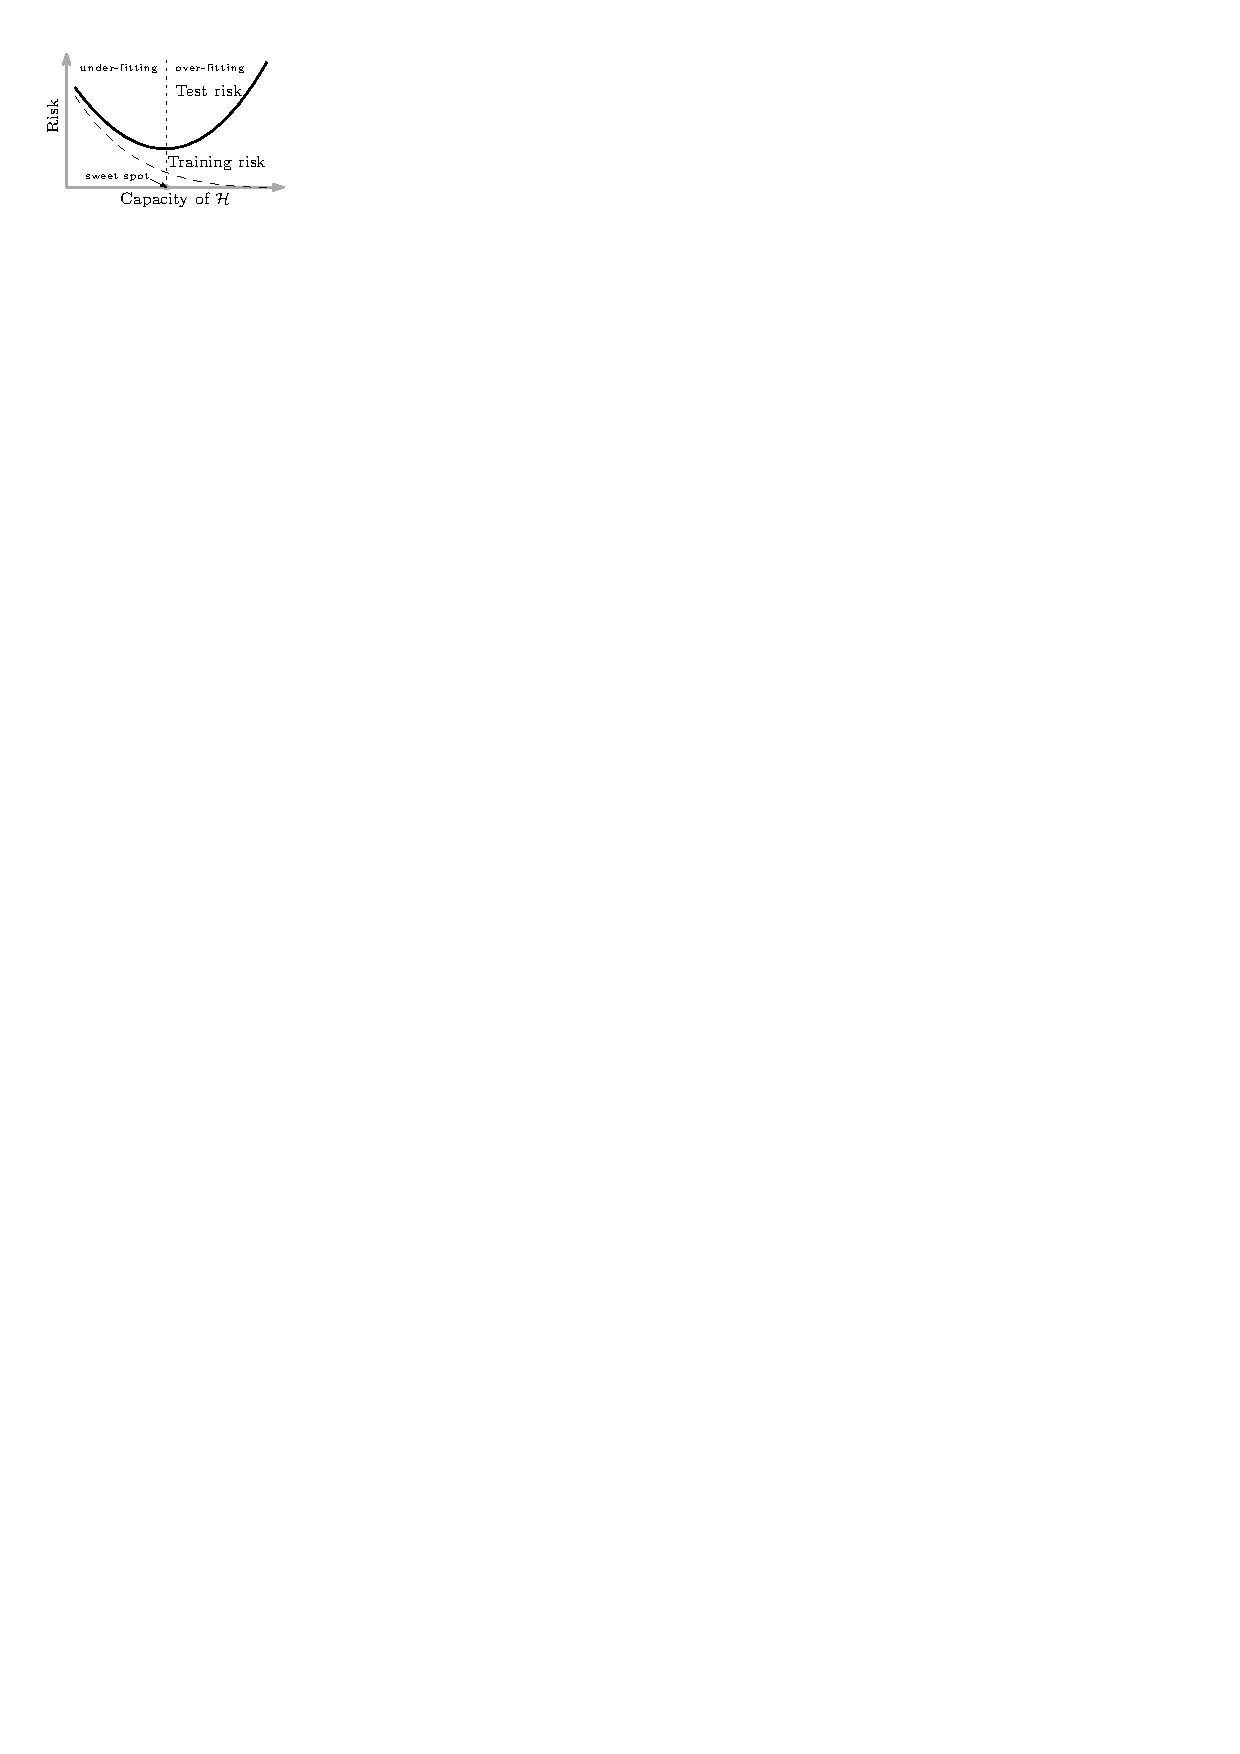
\includegraphics[height=0.13\textheight]{pdf/u-shaped.pdf} &
    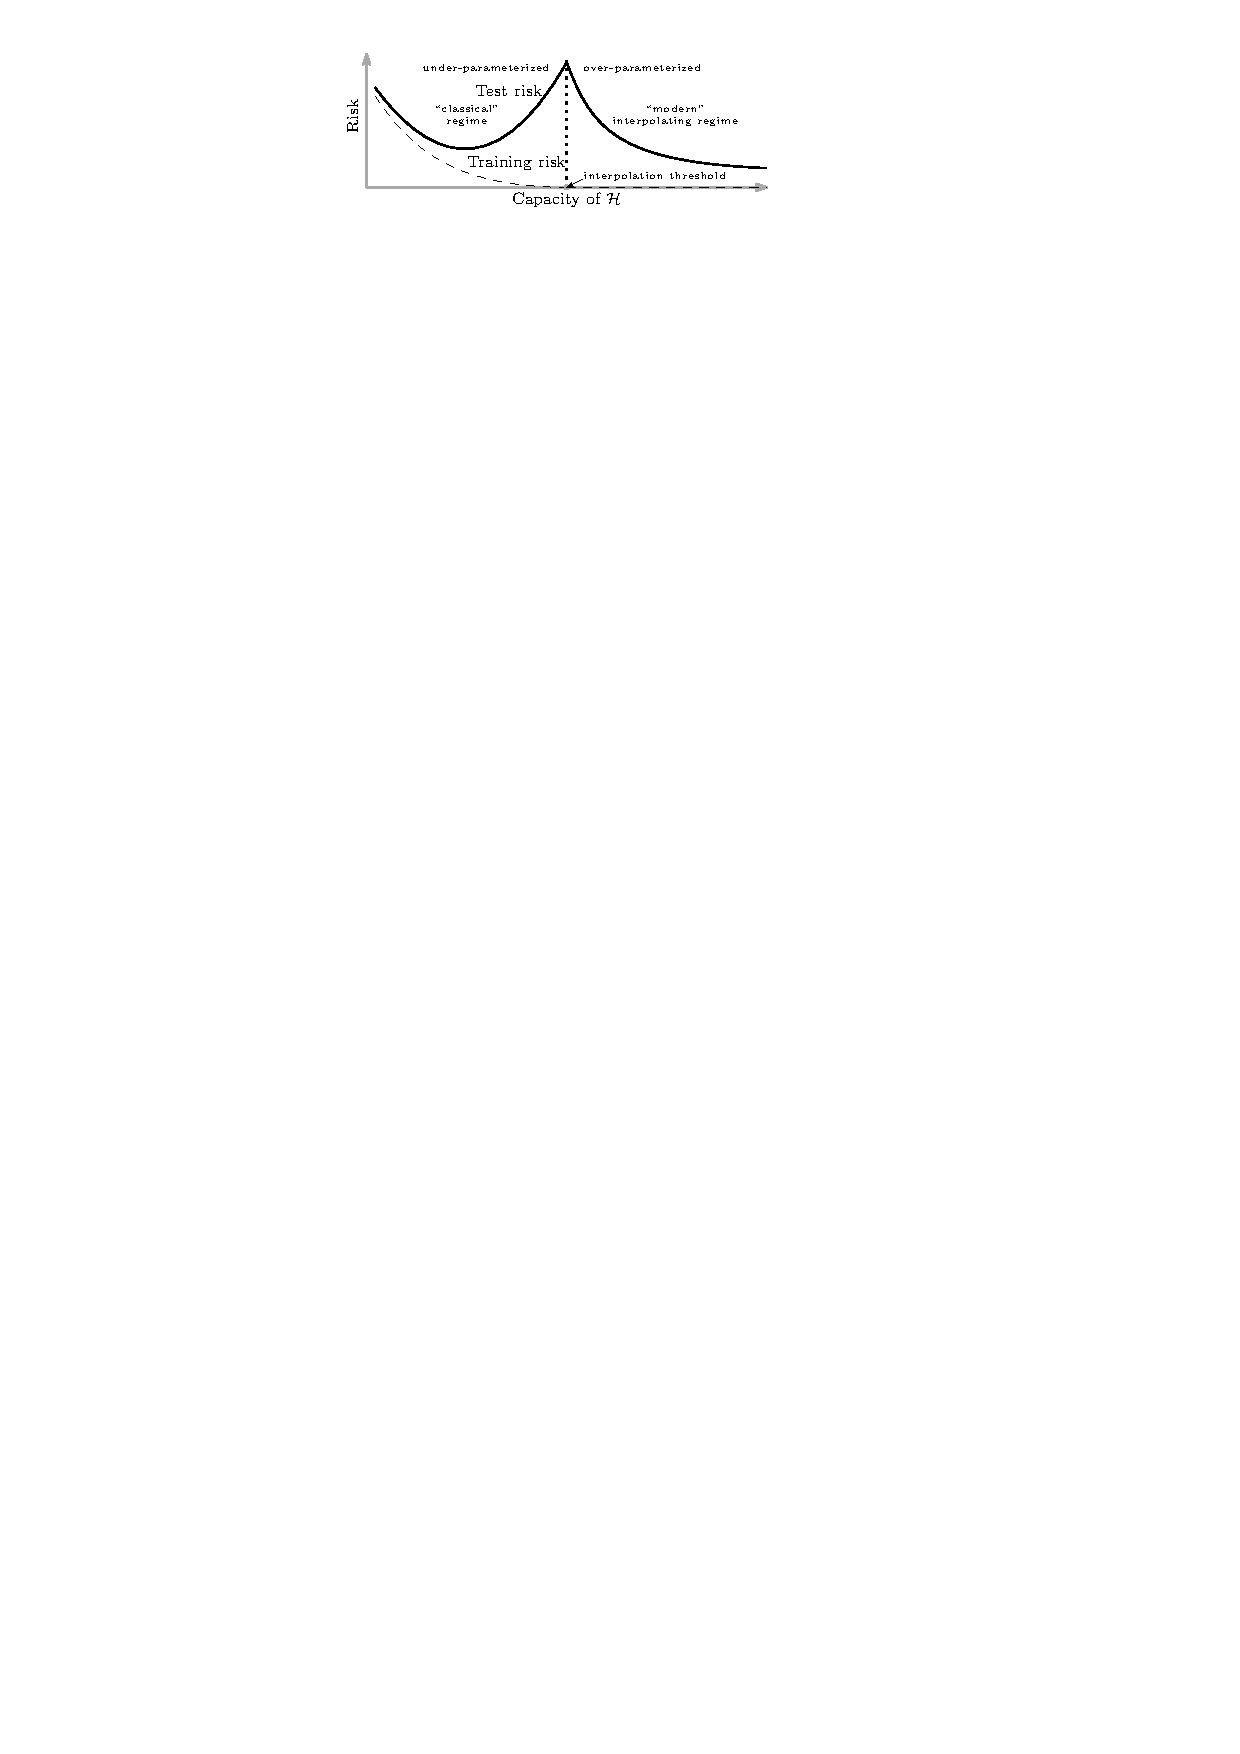
\includegraphics[height=0.13\textheight]{pdf/doubledescent.pdf} \\
    {\bf (a)} & {\bf (b)}
    \end{tabular}
    \caption{{\bf Curves for training risk (dashed line) and test risk (solid line).}
      ({\bf a}) The classical \emph{U-shaped risk curve} arising from the bias-variance trade-off.
      ({\bf b}) The \emph{double descent risk curve}, which incorporates the U-shaped risk curve (i.e., the ``classical'' regime) together with the observed behaviour from using high capacity function classes (i.e., the ``modern'' interpolating regime), separated by the interpolation threshold.
      The predictors to the right of the interpolation threshold have zero training risk. Reproduced from \cite{belkin_reconciling_2019}.}
    \label{fig:double-descent}
\end{figure}

The main finding that Belkin found is a pattern for how the apparent performance on unseen data depends on model capacity and the mechanism underlying the emergence of double descent. When function class capacity is below the "interpolation threshold", learned predictors exhibit the classical $U$-shaped curve from Figure~\ref{fig:double-descent}. The `modern' interpolating regime marks the opposite trend to the right, where the risk starts to decrease up to a lower bound, which then can be called the \textit{optimal descent bound}. 

\blockquote[\cite{belkin_reconciling_2019}]{The bottom of the $U$ is achieved at the sweet spot which balances the fit to the training data and the susceptibility to over-fitting:
to the left of the sweet spot, predictors are under-fit, and immediately to the right, predictors are over-fit.
When we increase the function class capacity high enough (e.g., by increasing the number of features or the size of the neural network architecture), the learned predictors achieve (near) perfect fits to the training data---i.e., interpolation.
Although the learned predictors obtained at the interpolation threshold typically have high risk, we show that increasing the function class capacity beyond this point leads to decreasing risk, typically going below the risk achieved at the sweet spot in the ``classical'' regime.}

Another prominent result to look at is \cite{nakkiran_deep_2019}, on the double descent of deep learning models. This is the first step toward identifying double descent to be perhaps, universal. 

\begin{figure}[htb]
    \centering
    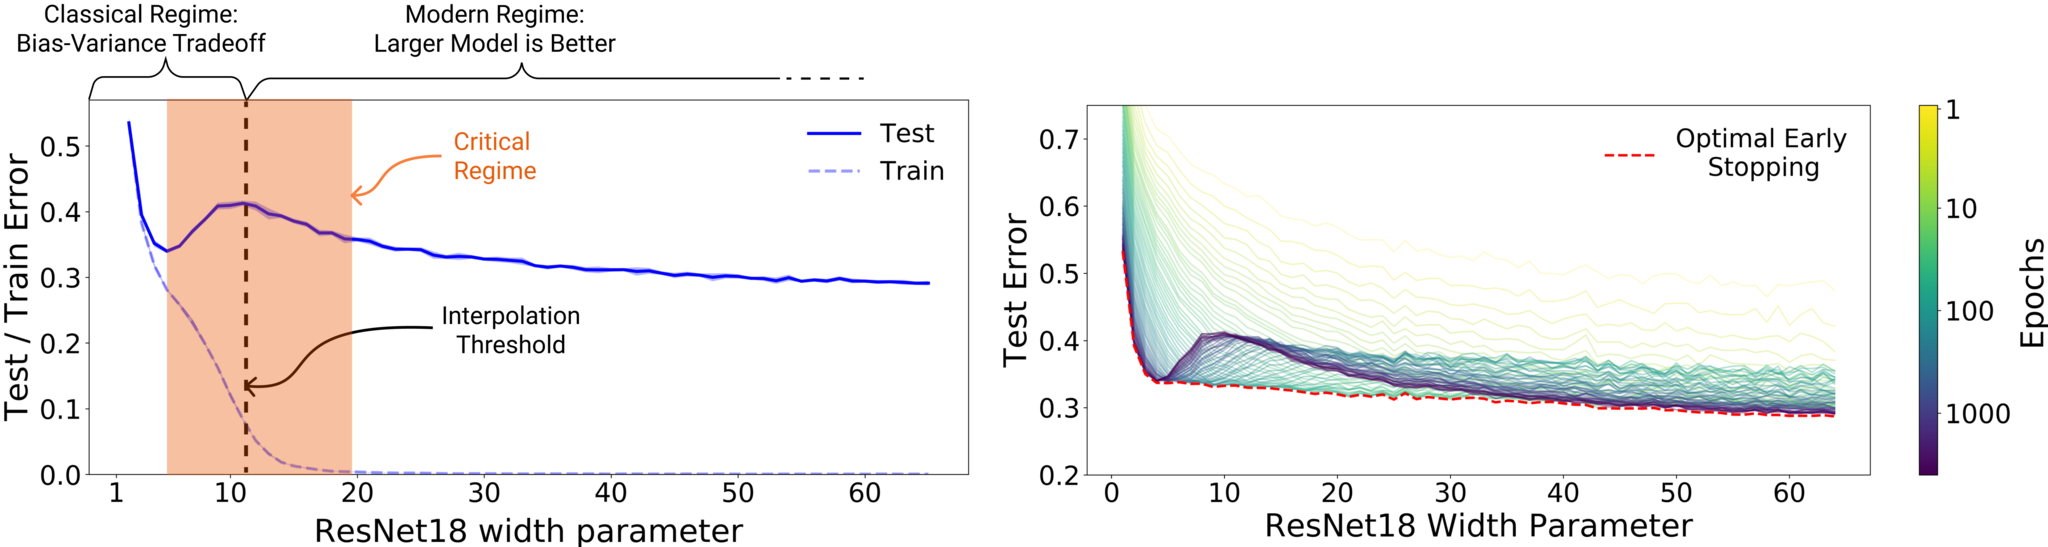
\includegraphics[width=1\textwidth]{media/errorvscomplexity.png}
    \caption{{\bf Left:} Train and test error as a function of model size,
    for ResNet18s of varying width 
    on CIFAR-10 with 15\% label noise.
    %In the under-parameterized regime, test error follows
    %the behavior predicted by classical statistical learning theory, but in the overparameterized regime (once training error is approximately zero),  the test error undergoes a ``second descent'' and decreases as model size increases. The shaded region represents the critically parameterized regime where the transition from under- to over-parameterization occurs. 
    {\bf Right:}
    Test error, shown for varying train epochs.
    %The dashed red line shows that with optimal early stopping double descent is not observed.
    % All models are ResNet18s of varying width,
    % trained on CIFAR10 with 15\% label noise
    All models trained using Adam for 4K epochs.
    %, and plotting means and standard-deviations from 5 trials with random network initialization.
    The largest model (width $64$) corresponds to standard ResNet18. Resued from \cite{nakkiran_deep_2019}.
    %    \ptodo{point out that interpolation point for second plot is plotted in the ocean plot}
    }
    \label{fig:errorvscomplexity}
\end{figure}

\begin{figure}[htb]
\centering
\begin{minipage}{.512\textwidth}
  \centering
  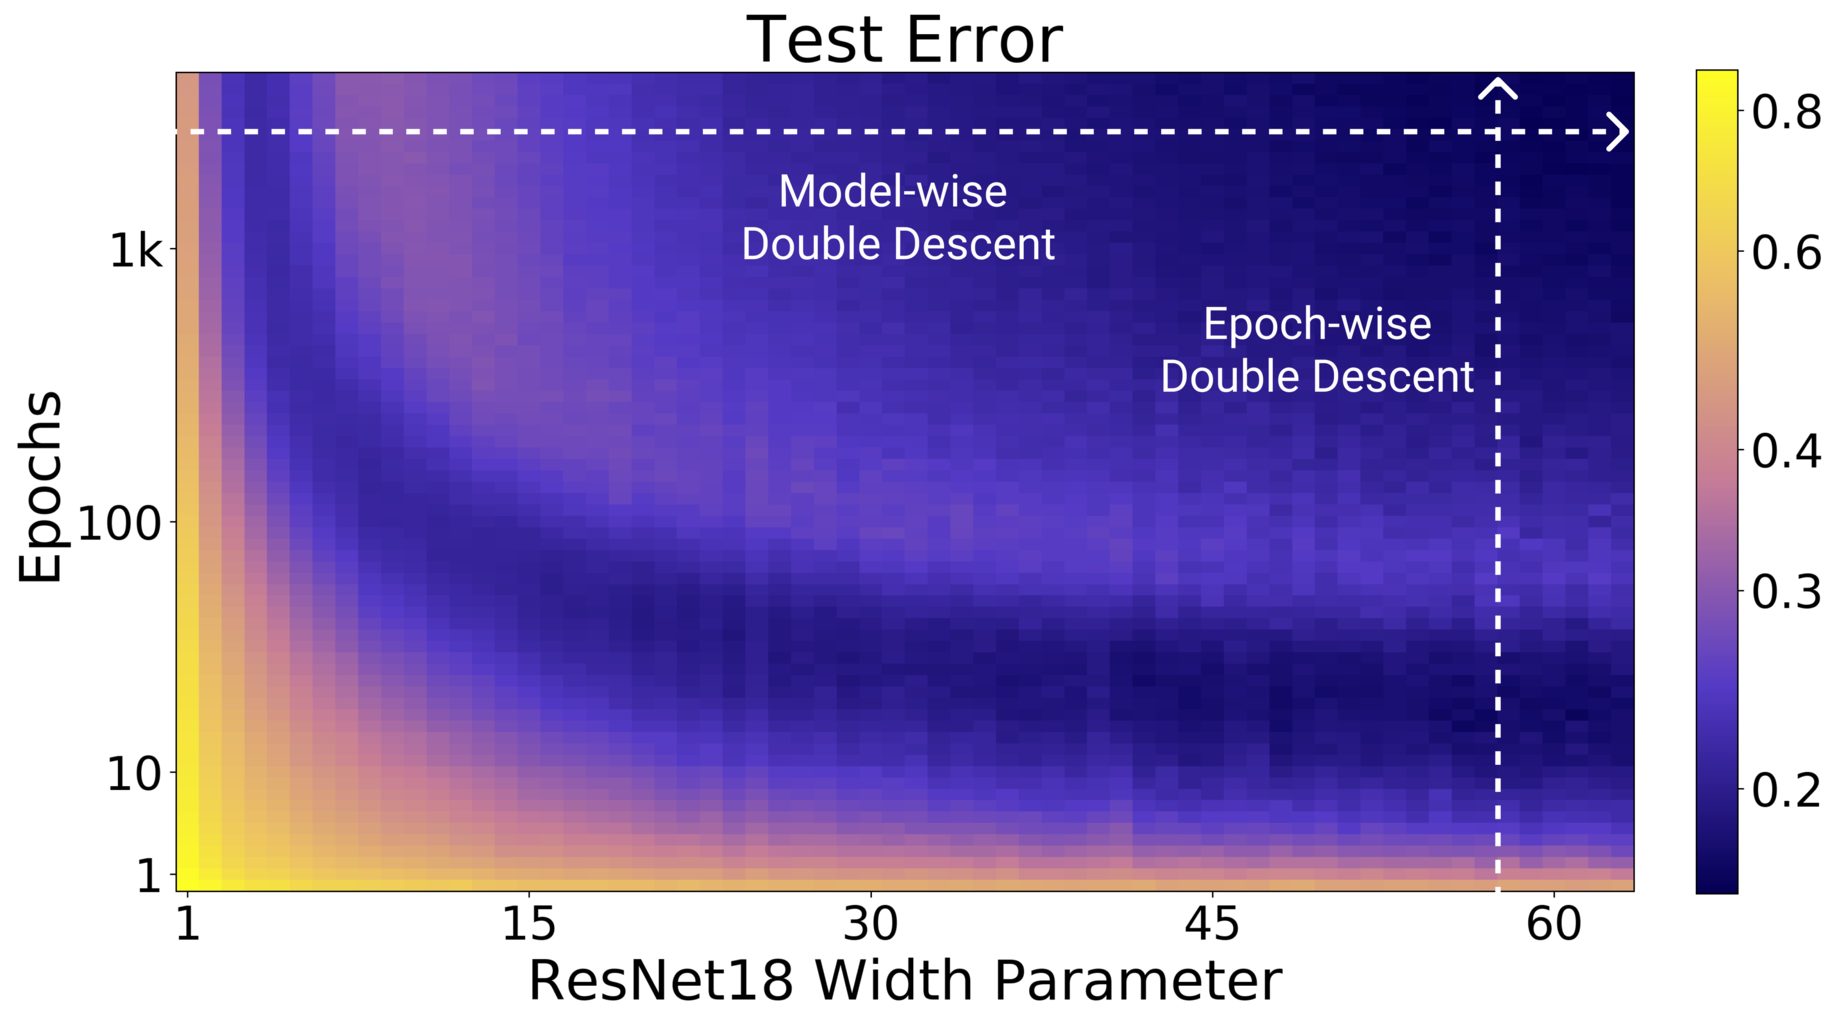
\includegraphics[width=1\textwidth]{media/Intro-ocean-test.png}
\end{minipage}%
\begin{minipage}{.488\textwidth}
  \centering
  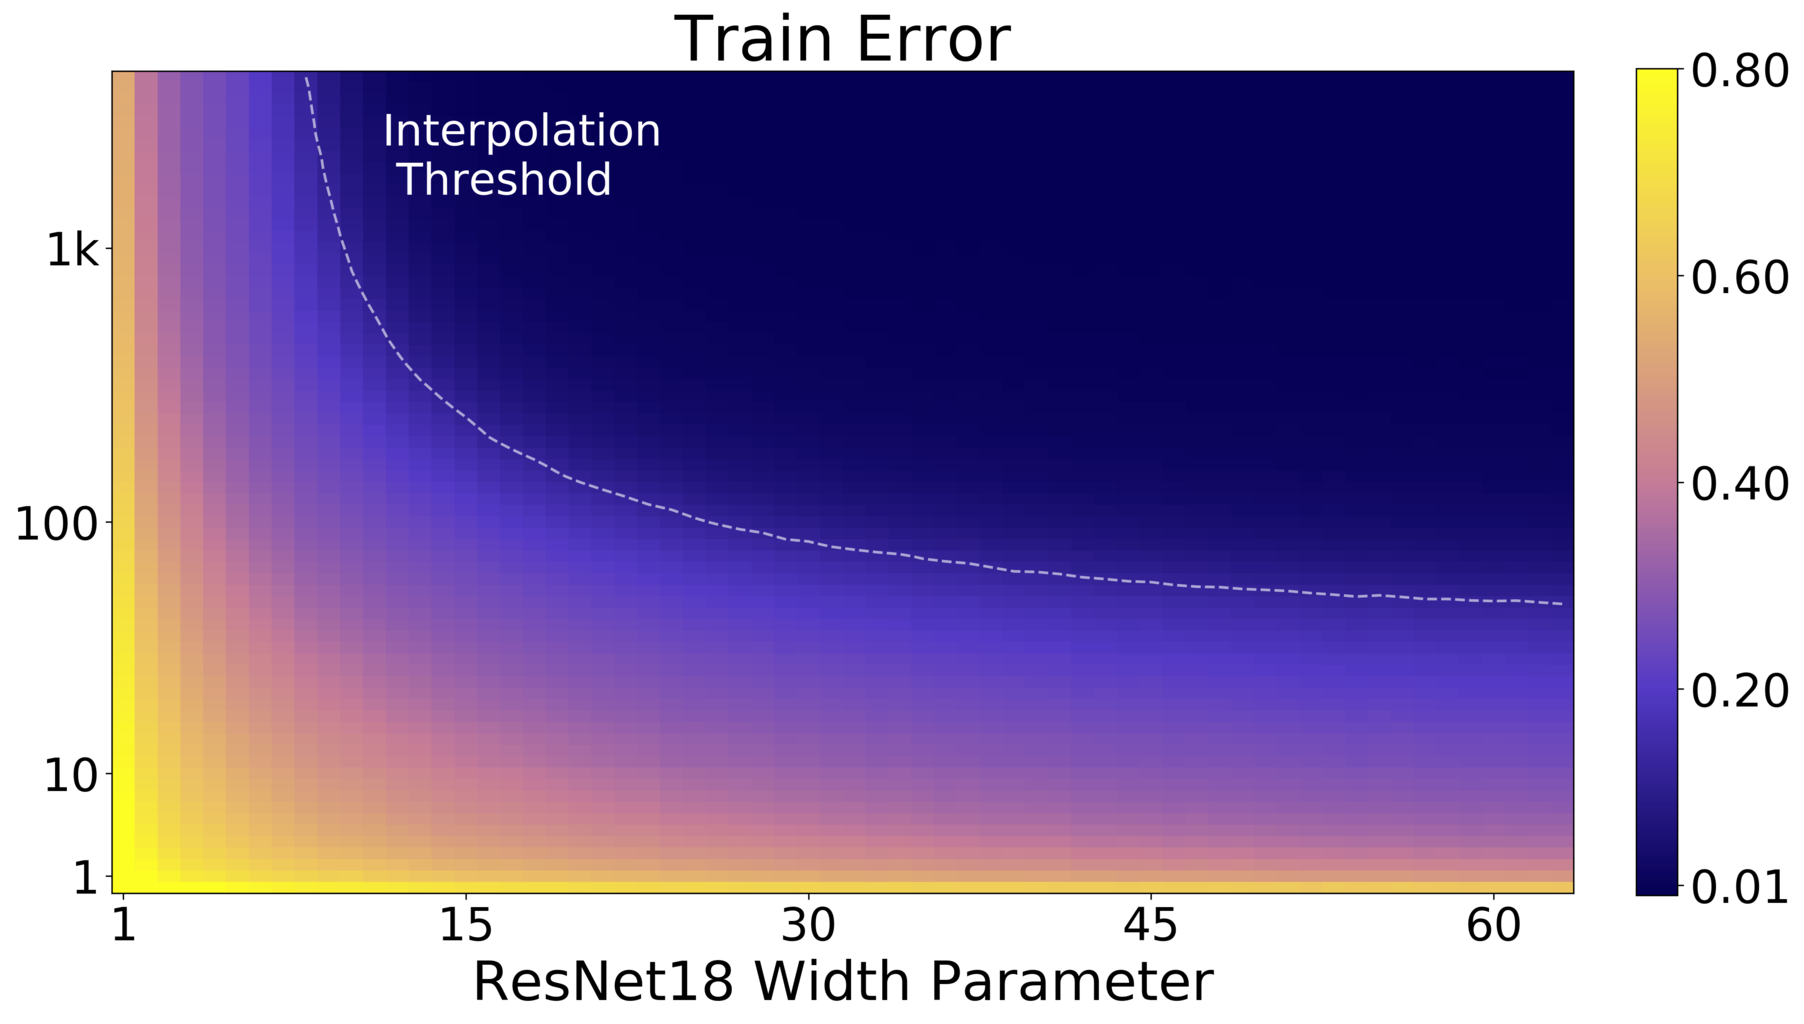
\includegraphics[width=1\textwidth]{media/Rn-cifar10-p15-adam-aug-train.png}
\end{minipage}
\caption{{\bf Left:} Test error as a function of model size and train epochs. The horizontal line corresponds to model-wise double descent--varying model size while training for as long as possible.
The vertical line corresponds to epoch-wise double descent,
with test error undergoing double-descent as train time increases.
{\bf Right} Train error of the corresponding models.
All models are Resnet18s trained on CIFAR-10 with 15\% label noise,
data-augmentation, and Adam for up to 4K epochs. Reused from \cite{nakkiran_deep_2019}}
\label{fig:unified}
\end{figure}

They define \emph{effective model complexity} of $\mathcal{T}$ (w.r.t. distribution $\mathcal D$) to be the maximum number of samples $n$ on which $\mathcal{T}$ achieves on average $\approx 0$ \emph{training error}. This is an entirely empirical definition, similarly per definition as VC-dimension. 

\newcommand{\EMC}{\mathrm{EMC}}
\begin{definition}[Effective Model Complexity]
The \emph{Effective Model Complexity} (EMC) of a training procedure $\cT$, with respect to distribution $\cD$ and parameter $\epsilon>0$,
is defined as:
\begin{align*}
    \EMC_{\cD,\eps}(\cT)
    :=  \max \left\{n ~|~ \E_{S \sim \cD^n}[ \mathrm{Error}_S( \cT( S )  ) ] \leq \eps \right\}
    \end{align*}
    where $\mathrm{Error}_S(M)$ is the mean error of model $M$ on train samples $S$.
\end{definition}

Using this definition, their main hypothesis can then be stated as the following three-fold regions:

\begin{hypothesis}[Generalized Double Descent hypothesis, informal] \label{hyp:informaldd}
For any natural data distribution $\cD$, neural-network-based training procedure $\cT$, and small $\epsilon>0$,
if we consider the task of predicting labels based on  $n$ samples from $\cD$ then:
\begin{description}
    \item[Under-parameterized regime.]  If~$\EMC_{\cD,\epsilon}(\cT)$ is sufficiently smaller than $n$, any perturbation of $\cT$ that increases its effective complexity will decrease the test error.
    \item[Over-parameterized regime.] If $\EMC_{\cD,\epsilon}(\cT)$ is sufficiently larger than $n$,
    any perturbation of $\cT$ that increases its effective complexity will decrease the test error.
    
    \item[Critically parameterized regime.] If $\EMC_{\cD,\epsilon}(\cT) \approx n$, then
    a perturbation of $\cT$ that increases its effective complexity
    might decrease {\bf or increase} the test error.
\end{description}
\end{hypothesis}

It is to notice that this definition is also only observational. By that, it only outlines the specific region of interest where the paradigm shift is identified through experimental results. It has no effective predictive power, or rather descriptive power more than setting up hypothesis with respect to the effective model complexity, and some arbitrary perturbation. \cite{nakkiran_deep_2019} also noticed this difficulty in providing a theoretical definition and theorem regarding such hypothesis, as said in their manuscript. The existence of the critical regime is also not defined. 

The behaviour itself has been particularly investigated, in certain settings. For example, before \cite{belkin_reconciling_2019}, \cite{advani2017highdimensionaldynamicsgeneralizationerror} investigated the generalization error in neural networks of high-dimensional measure. Of such, various behaviours that bear similarity to double descent can be observed. \cite{belkin2018understanddeeplearningneed} expanded on his previous research on the particular subset of kernel learning models, providing a theoretical analysis of specifically the Laplacian kernel on standard neural network. \cite{mei2020generalizationerrorrandomfeatures} investigated random feature regression in such regard, and also found similar results. 

The fact that double descent is not well-defined itself is a problem on its own. Up to the author's knowledge and of myself, there has been no effective definition or given description that outlines specifically how double descent can be structured. Instability in reproducing experiments and the effective range of the phenomena remains a question on its own. 

\clearpage

\bibliography{references}
\bibliographystyle{iclr2025_conference}

\clearpage



\end{document}
